\documentclass[11pt,a4paper,roman]{scrartcl}
\usepackage{parskip}
\usepackage[english]{babel}
\usepackage{url}
\usepackage[utf8x]{inputenc}
\usepackage{amsmath}
\usepackage{amssymb}
\usepackage{graphicx}
\usepackage[export]{adjustbox}
\usepackage{listings}
\usepackage{float}
\usepackage{hyperref}
\usepackage[document]{ragged2e}
\usepackage{bm}
\usepackage[section]{placeins}
\title{Computer exercise 5}
\date{}
\author{Carl Ridnert, 940325-0112, ridnert@kth.se \\
Yue Jiao, 911024-7799, yj@kth.se}


\begin{document}
\maketitle
\begin{figure}[h]
\centering
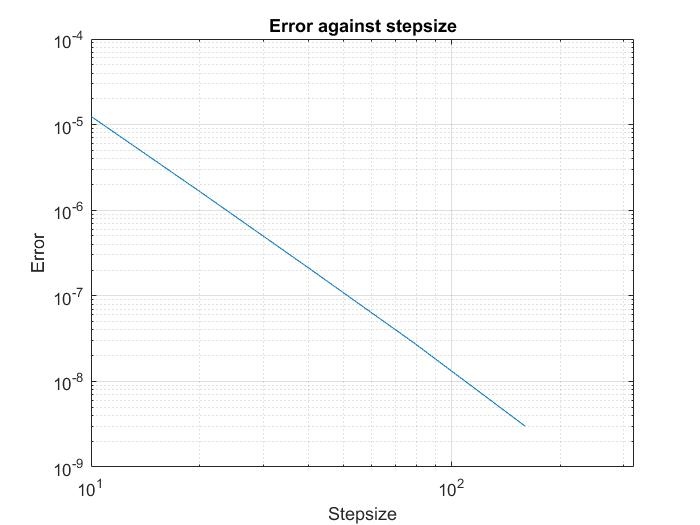
\includegraphics[width=0.45\textwidth,center]{1}
\end{figure}
\newpage

\section*{Problem description}
In this exercise, the following PDE is solved using.
\begin{equation}
\begin{aligned}
-\Delta T = f\textrm{, } \quad (x,y) \in [0\leq x \leq 4, 0 \leq y \leq 2 ] \\
T(0,y)=300 \textrm{, } \quad T(4,y)=600 \textrm{, } \quad 0 \leq y \leq 2 \\
\frac{\partial T}{\partial y}(x,0)=0 \textrm{, } \quad \frac{\partial T}{\partial y}(x,2)=0 \textrm{, } \quad 0 \leq x \leq 4 \\
\end{aligned}
\end{equation}
This models the heat conduction in a rectangular plate where the boundary conditions are such that the top and bottom are isolated and the right and left have a constant temperature. The problem is solved with two different force function $f=0$ and $f=1500\cdot \exp(-5(x-2)^2-10(y-0.5)^2)$.

\section*{1}
The finite difference method is used for this problem set up. The x-axis of the domain is discretized into N nodes and the y-axis is discretized into M nodes. The step-size $h=x_i-x_{i-1}=y_j-y_{j-1}$ is the same in both x- and y-direction. Let $u$ be the discretization of function $T$ so that for node $(x_i, y_j)$, $T(x_i, y_j) = u_{i,j}$. 

With the discretization, the Laplace operator $\Delta$ of the temperature can be written as: 
\begin{equation}
\begin{aligned}
-\Delta T & = -\frac{u_{i-1,j} - 2u_{i,j} + u_{i+1,j}}{h^2}-\frac{u_{i,j-1} - 2u_{i,j} + u_{i,j+1}}{h^2} \\
& = \frac{1}{h^2}\left( 4u_{i,j} - u_{i-1,j} - u_{i+1,j} - u_{i,j-1} - u_{i,j+1} \right)
\end{aligned}
\end{equation}

Since we have a Dirichlet boundary conditions on $x=0$ and $x=4$, no nodes are defined on the boundaries $x=0$ and $x=4$. The boundary conditions on $y=0$ and $y=2$ are Neumann condition, this implies that nodes needs to be defined on those boundaries. This means that thee coordinates are of the form $x_i = ih, i\in \{1,...,N\}$ and $y_j = h(j-1), j\in \{1,..., M\}$ where $(N+1)h=4$ and $(M-1)h = 2$. 

In order to have second order accuracy, ghost points are added outside all boundaries so that we have $x_0 = 0$, $x_{N+1}=4$, $y_0 = -h$ and $y_{M+1} = 2+h$. Thus the Dirichlet boundary conditions imply the following: 
\begin{equation}
\begin{aligned}
T(0, y) = u_{0,j}=300 \textrm{, } \quad T(4,y) = u_{N+1, j} = 600
\end{aligned}
\end{equation}

The Neumann boundary conditions imply that: 
\begin{equation}
\begin{aligned}
\frac{\partial T}{\partial y}(x,0)=\frac{u_{i,2}-u_{i,0}}{2h} = 0 \quad & \Rightarrow \quad u_{i,2}=u_{i,0} \\
\frac{\partial T}{\partial y}(x,2)=\frac{u_{i,M+1}-u_{i,M-1}}{2h}=0 \quad & \Rightarrow \quad u_{i,M+1}=u_{i,M-1} 
\end{aligned}
\end{equation}

With these boundary conditions, the Laplace equation on the boundary can be expressed as the following system of $N\cdot M$ equations: 
\begin{equation}
\begin{aligned}
-\Delta T(0, 0) & = \frac{1}{h^2}\left( 4u_{1,1} - 300 - u_{2,1} - 2u_{1,2} \right) \\
-\Delta T(4, 0) & = \frac{1}{h^2}\left( 4u_{N,1} - 600 - u_{N-1,1} - 2u_{N,2} \right) \\
-\Delta T(0, 2) & = \frac{1}{h^2}\left( 4u_{1,M} - 300 - u_{2,M} - 2u_{1,M-1} \right) \\
-\Delta T(4, 2) & = \frac{1}{h^2}\left( 4u_{N,M} - 600 - u_{N-1,M} - 2u_{N,M-1} \right) \\
-\Delta T(0, y) & = \frac{1}{h^2}\left( 4u_{1,j} - 300 - u_{2,j} - u_{1,j-1} - u_{1,j+1} \right) \\
-\Delta T(4, y) & = \frac{1}{h^2}\left( 4u_{N,j} - 600 - u_{N-1,j} - u_{N,j-1} - u_{N,j+1} \right) \\
-\Delta T(x, 0) & = \frac{1}{h^2}\left( 4u_{i,1} - 2u_{i,2} - u_{i-1,1} - u_{i+1,1} \right) \\
-\Delta T(x, 2) & = \frac{1}{h^2}\left( 4u_{i,M} - 2u_{i,M-1} - u_{i-1,M} - u_{i+1,M} \right) \\
\end{aligned}
\end{equation}

With these relationships, the PDE can be rewritten in the matrix form $Av +b = f$. Where matrix $A$ is a band matrix with bandwidth N+1 and describes the linear relationships between the values of $u_{i,j}$, $v$ contains the $u_{i,j}s$  and vector $b$ is the vector that describe the Dirichlet boundary conditions that can not be fitted in the $A$ matrix.

The solutions to (1) is computed using with this method using two different values of the step size. Plots of the temperature over the rectangular domain is shown below:

\begin{figure}[h]
\centering
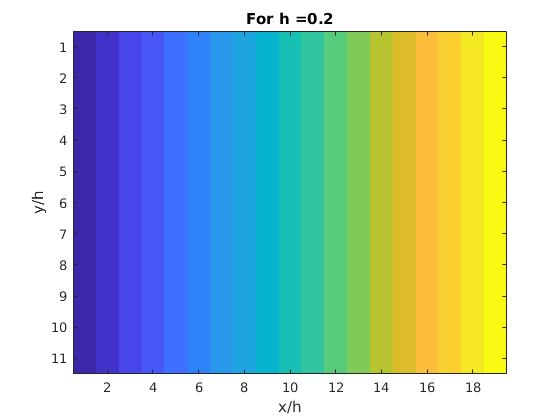
\includegraphics[width=0.6\textwidth,center]{plot3}
\caption{Solution in the case where f=0 and h=0.2}
\end{figure}
Here, a more yellow color corresponds to a higher temperature.
\begin{figure}[!htbp]
\centering
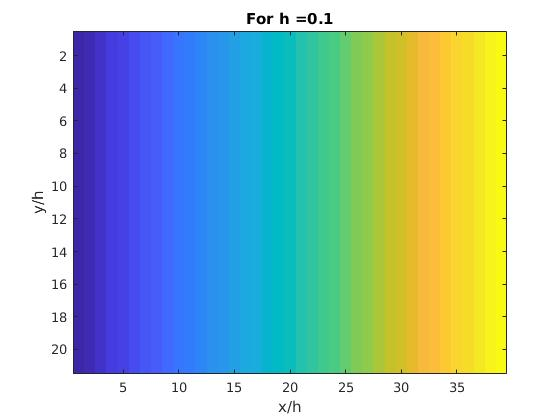
\includegraphics[width=0.6\textwidth,center]{plot1}
\caption{Solution where f=0 and h=0.1}
\end{figure}

The value at $(x,y)=(2,1)$ is 450 degrees. 


Note that this solution is apparently only dependent of x. Thus, one can realize that the exact solution is a linear function over the x-axis. More specifically, a function that can be written as.
\begin{equation}
T(x)=300+75x, x\in [0,4]
\end{equation}


Now lets define the function f as

\begin{equation}
          f=1500*exp(-5(x-2)^2-10(y-0.5)^2)
          \label{Eq1}
\end{equation}

Then the numerical solution to (1) can be depicted as in figure 3 and 4 below. For this definition of f, the value at $(x,y)=(2,1)$ equals approximately 730 degrees with a deviation of one degree between the solutions using different step sizes. 

\begin{figure}[h]
\centering
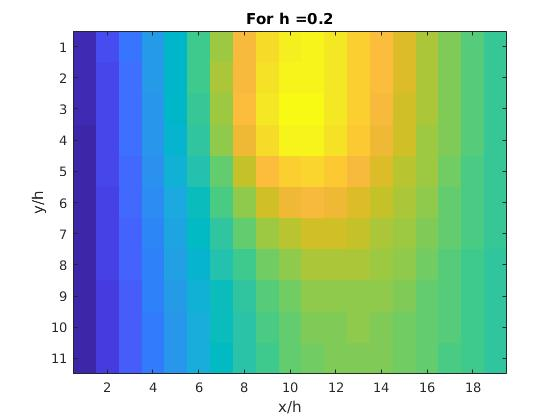
\includegraphics[width=0.6\textwidth,center]{plot4}
\caption{Solution where f is as given in equation $(7)$ and h=0.2}
\end{figure}

\begin{figure}[h]
\centering
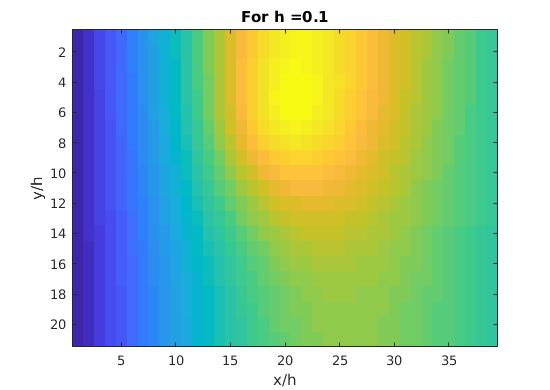
\includegraphics[width=0.6\textwidth,center]{plot2}
\caption{Solution where f is as given in equation $(7)$ and h=0.1}
\end{figure}

The solution is no longer linear in x and constant in y so it is very hard to see what an exact solution would look like.

\section*{2}
Here we use Comsol simulation to solve the same PDE problem as above for $f=1500*exp(-5(x-2)^2-10(y-0.5)^2)$. 
Two different mesh sizes are used and values of point $(2,1)$ correspond to these two meshes are calculated. 
The results are shown below, note that the plots in Comsol are flipped compared to the ones produced in section one, however it appears as they agree on the result. 

\begin{figure}[!h]
\centering
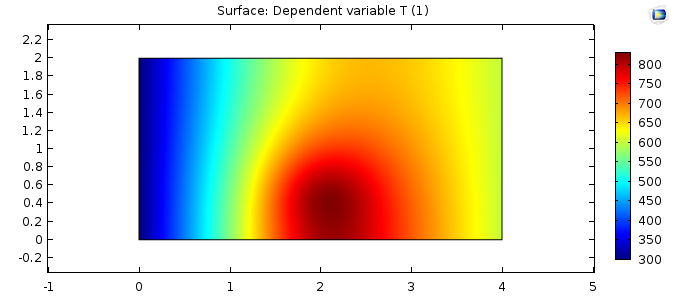
\includegraphics[width=0.6\textwidth,center]{comsol_1}
\caption{Solution done by Comsol with Normal mesh size}
\end{figure}
This mesh size gives 679 degrees of freedom and the value at $(2,1)$ is $731.41$. 

\begin{figure}[H]
\centering
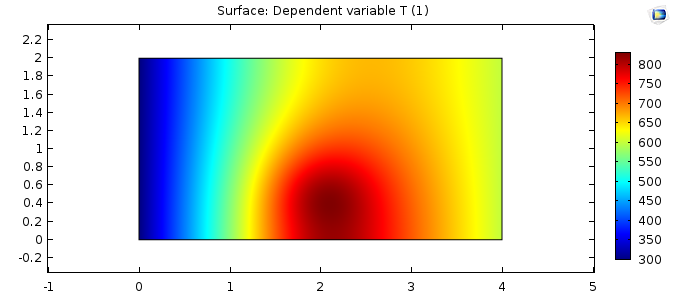
\includegraphics[width=0.6\textwidth,center]{comsol_2}
\caption{Solution done by Comsol with Fine mesh size}
\end{figure}
This mesh size gives 1011 degrees of freedom and the value at $(2,1)$ is $731.45$. 

\newpage
\section*{3}
In this problem, the domain is changed to an L shape and is studied with Comsol, the geometry along with the solution is shown in figure 7. The same force function $f$ is used and different mesh sizes are tested. 

\begin{figure}[H]
% \centering
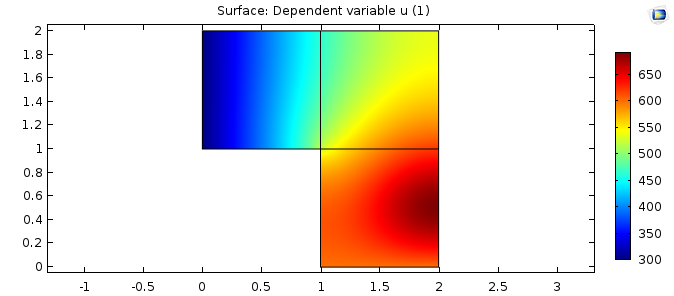
\includegraphics[width=0.6\textwidth,center]{comsol_3}
\caption{Solution done by Comsol with x- and y-direction scale equal with 1}
\end{figure}
This mesh size gives 1061 degrees of freedom. The value at $(1,1)$ is $523.56$ and the value at $(2,2)$ is $536,74$. The mesh is showed below. 

\begin{figure}[H]
% \centering
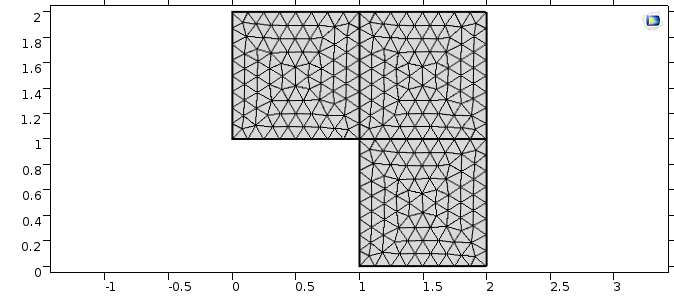
\includegraphics[width=0.6\textwidth,center]{comsol_32}
\caption{The mesh when x- and y-direction scale equal with 1}
\end{figure}


\begin{figure}[H]
% \centering
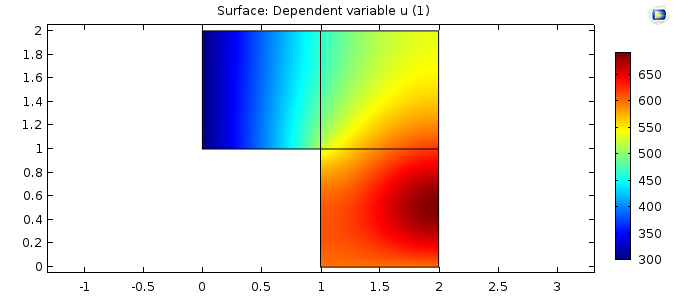
\includegraphics[width=0.6\textwidth,center]{comsol_4}
\caption{Solution done by Comsol with x- and y-direction scale equal with 2}
\end{figure}
This mesh size gives 3601 degrees of freedom. The value at $(1,1)$ is $523.56$ and the value at $(2,2)$ is $536,74$. The mesh is showed below. 

\begin{figure}[H]
% \centering
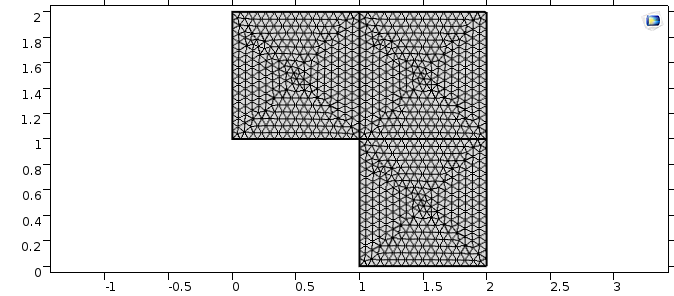
\includegraphics[width=0.6\textwidth,center]{comsol_42}
\caption{The mesh when x- and y-direction scale equal with 2}
\end{figure}


\begin{figure}[H]
% \centering
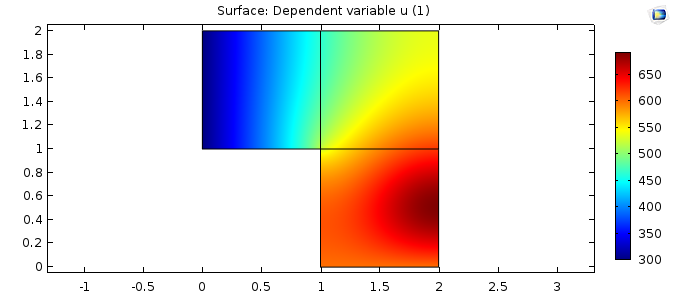
\includegraphics[width=0.6\textwidth,center]{comsol_5}
\caption{Solution done by Comsol with refinement near point $(2,2)$}
\end{figure}
This mesh size gives 2123 degrees of freedom. The value at $(1,1)$ is $523.70$ and the value at $(2,2)$ is $536,74$. The mesh is showed below. 

\begin{figure}[H]
%\centering
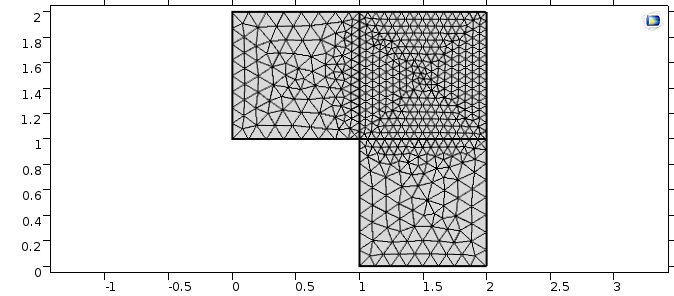
\includegraphics[width=0.6\textwidth,center]{comsol_52}
\caption{The mesh after refinement}
\end{figure}

Note that the solution does not vary much when the mesh size is increased. 


\end{document}




clc,clear all,close all

%% Computer Exercise 5

%Solving Elliptic PDE for heat transfer
%Plate where 0<=x<=4, 0<=y<=2


%Step size

for h=[0.1 0.2];

%Number of steps
%x
N=4/h-1;
%y
M=2/h+1;



%Building A matrix
In = eye(N,N);
Sm=[];
for i = 2:M-1
    
    Sm(i,i)=2;
    Sm(i,i+1)=-1;
    Sm(i,i-1)=-1;
    
end
Sm(1,1)=2;
Sm(1,2)=-1;
Sm(M,M)=2;
Sm(M,M-1)=-1;

Im=eye(M,M);

Sn= [];
for i = 2:N-1
    
    Sn(i,i)=2;
    Sn(i,i+1)=-1;
    Sn(i,i-1)=-1;
    
end
Sn(1,1)=2;
Sn(1,2)=-1;
Sn(N,N)=2;
Sn(N,N-1)=-1;

A=kron(Im,Sn)+kron(Sm,In);

%Working with (BC)

%ui,0=ui,2
%ui,M+1=ui,M-1
%Gives the following modifications in the A matrix
for k=1:N
A(k,k+N)=-2;
end
 for i=M*N-N+1:N*M
     A(i,i-N)=-2;
 end
 
 
 
 %B-matrix %Dirchlet Conditions
 %u0,i=300 uN+1,i=600
 b=[];
 for i=1:N:N*M
     b(i)=300;
     b(i+N-1)=600;
 end
 
 f=[];
 
 for j=1:M
     for i = 1:N
         f(i+(j-1)*N) = 1500*exp(-5*(i*h-2)^2-10*((j-1)*h-0.5)^2);
     end
 end

 b2=h^2*f+b;
 
 
 %Solve
 
 u=A\b';
 
 u2=A\b2';
 
 U=[];
 U2=[];
 %Sorting u
 for j=1:M
     
 U(:,j)=u(j*N-N+1:j*N);
 
 U2(:,j)=u2(j*N-N+1:j*N);
 end
 
 
 
 
 
 figure
  imagesc(U')   
 xlabel('x/h')
 ylabel('y/h')
 title(['For h =' num2str( h)])
 figure
 imagesc(U2')
 xlabel('x/h')
 ylabel('y/h')
 title(['For h =' num2str( h)])
 
end
 
 